\chapter{Theoretische Einführungen}

\section{Oberflächenplasmonenpolaritonen}%~\label{sec:spps}

Oberflächenplasmonenpolaritonen (engl. surface plasmon polaritons, SPPs)
sind elektromagnetische Anregungen/Wellen welche sich entlang der Grenzfläche 
zwischen Leiter und Dielektrikum ausbreiten.~\cite{plasmonics}
\begin{figure}
    \centering
    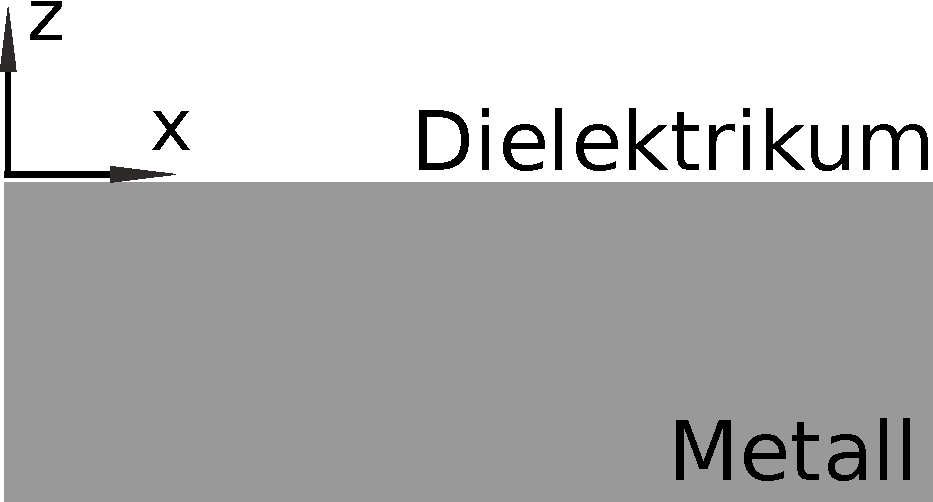
\includegraphics[scale=0.5]{./Plots/leiter_und_nichtleiter.pdf}
    \caption{Erkennbar sind die unterschiedlichen Schichten der Probe.
    Die unterste Schicht, das Substrat (hier schwarz) besteht aus Galliumarsenid (GaAs).}
    \label{fig:kasten}
\end{figure}
\FloatBarrier

Quantenmechanisch können diese als Quasiteilchen behandelt werden. 
Also als ein Phänomen was ein Teilchencharakter besitzt bzw. einer zugeordnet werden kann. 
Weitere Eigenschaft der SPPs sind ihr evaneszentes Verhalten bezogen auf das
durchdringen der Grenzfläche.
Der theoretische Zuganz zu SPPs gelingt über die Maxwellgleichungen.